\documentclass[1p]{elsarticle_modified}
%\bibliographystyle{elsarticle-num}

%\usepackage[colorlinks]{hyperref}
%\usepackage{abbrmath_seonhwa} %\Abb, \Ascr, \Acal ,\Abf, \Afrak
\usepackage{amsfonts}
\usepackage{amssymb}
\usepackage{amsmath}
\usepackage{amsthm}
\usepackage{scalefnt}
\usepackage{amsbsy}
\usepackage{kotex}
\usepackage{caption}
\usepackage{subfig}
\usepackage{color}
\usepackage{graphicx}
\usepackage{xcolor} %% white, black, red, green, blue, cyan, magenta, yellow
\usepackage{float}
\usepackage{setspace}
\usepackage{hyperref}

\usepackage{tikz}
\usetikzlibrary{arrows}

\usepackage{multirow}
\usepackage{array} % fixed length table
\usepackage{hhline}

%%%%%%%%%%%%%%%%%%%%%
\makeatletter
\renewcommand*\env@matrix[1][\arraystretch]{%
	\edef\arraystretch{#1}%
	\hskip -\arraycolsep
	\let\@ifnextchar\new@ifnextchar
	\array{*\c@MaxMatrixCols c}}
\makeatother %https://tex.stackexchange.com/questions/14071/how-can-i-increase-the-line-spacing-in-a-matrix
%%%%%%%%%%%%%%%

\usepackage[normalem]{ulem}

\newcommand{\msout}[1]{\ifmmode\text{\sout{\ensuremath{#1}}}\else\sout{#1}\fi}
%SOURCE: \msout is \stkout macro in https://tex.stackexchange.com/questions/20609/strikeout-in-math-mode

\newcommand{\cancel}[1]{
	\ifmmode
	{\color{red}\msout{#1}}
	\else
	{\color{red}\sout{#1}}
	\fi
}

\newcommand{\add}[1]{
	{\color{blue}\uwave{#1}}
}

\newcommand{\replace}[2]{
	\ifmmode
	{\color{red}\msout{#1}}{\color{blue}\uwave{#2}}
	\else
	{\color{red}\sout{#1}}{\color{blue}\uwave{#2}}
	\fi
}

\newcommand{\Sol}{\mathcal{S}} %segment
\newcommand{\D}{D} %diagram
\newcommand{\A}{\mathcal{A}} %arc


%%%%%%%%%%%%%%%%%%%%%%%%%%%%%5 test

\def\sl{\operatorname{\textup{SL}}(2,\Cbb)}
\def\psl{\operatorname{\textup{PSL}}(2,\Cbb)}
\def\quan{\mkern 1mu \triangleright \mkern 1mu}

\theoremstyle{definition}
\newtheorem{thm}{Theorem}[section]
\newtheorem{prop}[thm]{Proposition}
\newtheorem{lem}[thm]{Lemma}
\newtheorem{ques}[thm]{Question}
\newtheorem{cor}[thm]{Corollary}
\newtheorem{defn}[thm]{Definition}
\newtheorem{exam}[thm]{Example}
\newtheorem{rmk}[thm]{Remark}
\newtheorem{alg}[thm]{Algorithm}

\newcommand{\I}{\sqrt{-1}}
\begin{document}

%\begin{frontmatter}
%
%\title{Boundary parabolic representations of knots up to 8 crossings}
%
%%% Group authors per affiliation:
%\author{Yunhi Cho} 
%\address{Department of Mathematics, University of Seoul, Seoul, Korea}
%\ead{yhcho@uos.ac.kr}
%
%
%\author{Seonhwa Kim} %\fnref{s_kim}}
%\address{Center for Geometry and Physics, Institute for Basic Science, Pohang, 37673, Korea}
%\ead{ryeona17@ibs.re.kr}
%
%\author{Hyuk Kim}
%\address{Department of Mathematical Sciences, Seoul National University, Seoul 08826, Korea}
%\ead{hyukkim@snu.ac.kr}
%
%\author{Seokbeom Yoon}
%\address{Department of Mathematical Sciences, Seoul National University, Seoul, 08826,  Korea}
%\ead{sbyoon15@snu.ac.kr}
%
%\begin{abstract}
%We find all boundary parabolic representation of knots up to 8 crossings.
%
%\end{abstract}
%\begin{keyword}
%    \MSC[2010] 57M25 
%\end{keyword}
%
%\end{frontmatter}

%\linenumbers
%\tableofcontents
%
\newcommand\colored[1]{\textcolor{white}{\rule[-0.35ex]{0.8em}{1.4ex}}\kern-0.8em\color{red} #1}%
%\newcommand\colored[1]{\textcolor{white}{ #1}\kern-2.17ex	\textcolor{white}{ #1}\kern-1.81ex	\textcolor{white}{ #1}\kern-2.15ex\color{red}#1	}

{\Large $\underline{12a_{0357}~(K12a_{0357})}$}

\setlength{\tabcolsep}{10pt}
\renewcommand{\arraystretch}{1.6}
\vspace{1cm}\begin{tabular}{m{100pt}>{\centering\arraybackslash}m{274pt}}
\multirow{5}{120pt}{
	\centering
	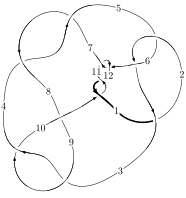
\includegraphics[width=112pt]{../../../GIT/diagram.site/Diagrams/png/1158_12a_0357.png}\\
\ \ \ A knot diagram\footnotemark}&
\allowdisplaybreaks
\textbf{Linearized knot diagam} \\
\cline{2-2}
 &
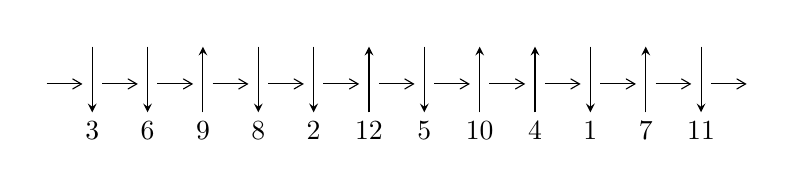
\begin{tikzpicture}[x=20pt, y=17pt]
	% nodes
	\node (C0) at (0, 0) {};
	\node (C1) at (1, 0) {};
	\node (C1U) at (1, +1) {};
	\node (C1D) at (1, -1) {3};

	\node (C2) at (2, 0) {};
	\node (C2U) at (2, +1) {};
	\node (C2D) at (2, -1) {6};

	\node (C3) at (3, 0) {};
	\node (C3U) at (3, +1) {};
	\node (C3D) at (3, -1) {9};

	\node (C4) at (4, 0) {};
	\node (C4U) at (4, +1) {};
	\node (C4D) at (4, -1) {8};

	\node (C5) at (5, 0) {};
	\node (C5U) at (5, +1) {};
	\node (C5D) at (5, -1) {2};

	\node (C6) at (6, 0) {};
	\node (C6U) at (6, +1) {};
	\node (C6D) at (6, -1) {12};

	\node (C7) at (7, 0) {};
	\node (C7U) at (7, +1) {};
	\node (C7D) at (7, -1) {5};

	\node (C8) at (8, 0) {};
	\node (C8U) at (8, +1) {};
	\node (C8D) at (8, -1) {10};

	\node (C9) at (9, 0) {};
	\node (C9U) at (9, +1) {};
	\node (C9D) at (9, -1) {4};

	\node (C10) at (10, 0) {};
	\node (C10U) at (10, +1) {};
	\node (C10D) at (10, -1) {1};

	\node (C11) at (11, 0) {};
	\node (C11U) at (11, +1) {};
	\node (C11D) at (11, -1) {7};

	\node (C12) at (12, 0) {};
	\node (C12U) at (12, +1) {};
	\node (C12D) at (12, -1) {11};
	\node (C13) at (13, 0) {};

	% arrows
	\draw[->,>={angle 60}]
	(C0) edge (C1) (C1) edge (C2) (C2) edge (C3) (C3) edge (C4) (C4) edge (C5) (C5) edge (C6) (C6) edge (C7) (C7) edge (C8) (C8) edge (C9) (C9) edge (C10) (C10) edge (C11) (C11) edge (C12) (C12) edge (C13) ;	\draw[->,>=stealth]
	(C1U) edge (C1D) (C2U) edge (C2D) (C3D) edge (C3U) (C4U) edge (C4D) (C5U) edge (C5D) (C6D) edge (C6U) (C7U) edge (C7D) (C8D) edge (C8U) (C9D) edge (C9U) (C10U) edge (C10D) (C11D) edge (C11U) (C12U) edge (C12D) ;
	\end{tikzpicture} \\
\hhline{~~} \\& 
\textbf{Solving Sequence} \\ \cline{2-2} 
 &
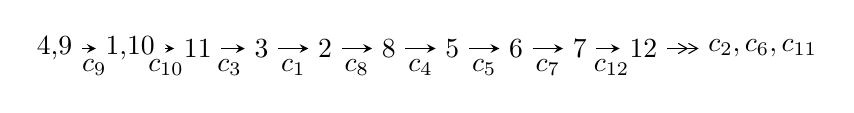
\begin{tikzpicture}[x=23pt, y=7pt]
	% node
	\node (A0) at (-1/8, 0) {4,9};
	\node (A1) at (17/16, 0) {1,10};
	\node (A2) at (17/8, 0) {11};
	\node (A3) at (25/8, 0) {3};
	\node (A4) at (33/8, 0) {2};
	\node (A5) at (41/8, 0) {8};
	\node (A6) at (49/8, 0) {5};
	\node (A7) at (57/8, 0) {6};
	\node (A8) at (65/8, 0) {7};
	\node (A9) at (73/8, 0) {12};
	\node (C1) at (1/2, -1) {$c_{9}$};
	\node (C2) at (13/8, -1) {$c_{10}$};
	\node (C3) at (21/8, -1) {$c_{3}$};
	\node (C4) at (29/8, -1) {$c_{1}$};
	\node (C5) at (37/8, -1) {$c_{8}$};
	\node (C6) at (45/8, -1) {$c_{4}$};
	\node (C7) at (53/8, -1) {$c_{5}$};
	\node (C8) at (61/8, -1) {$c_{7}$};
	\node (C9) at (69/8, -1) {$c_{12}$};
	\node (A10) at (11, 0) {$c_{2},c_{6},c_{11}$};

	% edge
	\draw[->,>=stealth]	
	(A0) edge (A1) (A1) edge (A2) (A2) edge (A3) (A3) edge (A4) (A4) edge (A5) (A5) edge (A6) (A6) edge (A7) (A7) edge (A8) (A8) edge (A9) ;
	\draw[->>,>={angle 60}]	
	(A9) edge (A10);
\end{tikzpicture} \\ 

\end{tabular} \\

\footnotetext{
The image of knot diagram is generated by the software ``\textbf{Draw programme}" developed by Andrew Bartholomew(\url{http://www.layer8.co.uk/maths/draw/index.htm\#Running-draw}), where we modified some parts for our purpose(\url{https://github.com/CATsTAILs/LinksPainter}).
}\phantom \\ \newline 
\centering \textbf{Ideals for irreducible components\footnotemark of $X_{\text{par}}$} 
 
\begin{align*}
I^u_{1}&=\langle 
1.53983\times10^{51} u^{99}+4.05833\times10^{51} u^{98}+\cdots+2.11035\times10^{51} b-1.02725\times10^{52},\\
\phantom{I^u_{1}}&\phantom{= \langle  }-1.15475\times10^{51} u^{99}-3.57142\times10^{51} u^{98}+\cdots+2.11035\times10^{51} a+1.63343\times10^{52},\;u^{100}+u^{99}+\cdots-4 u+4\rangle \\
I^u_{2}&=\langle 
u^3+2 b+2 a-2 u,\;-2 u^3 a+2 u^2 a- u^3+2 a^2+u^2-2 a+2 u-4,\;u^4-2 u^2+2\rangle \\
\\
I^v_{1}&=\langle 
a,\;b- v-1,\;v^2+v+1\rangle \\
\end{align*}
\raggedright * 3 irreducible components of $\dim_{\mathbb{C}}=0$, with total 110 representations.\\
\footnotetext{All coefficients of polynomials are rational numbers. But the coefficients are sometimes approximated in decimal forms when there is not enough margin.}
\newpage
\renewcommand{\arraystretch}{1}
\centering \section*{I. $I^u_{1}= \langle 1.54\times10^{51} u^{99}+4.06\times10^{51} u^{98}+\cdots+2.11\times10^{51} b-1.03\times10^{52},\;-1.15\times10^{51} u^{99}-3.57\times10^{51} u^{98}+\cdots+2.11\times10^{51} a+1.63\times10^{52},\;u^{100}+u^{99}+\cdots-4 u+4 \rangle$}
\flushleft \textbf{(i) Arc colorings}\\
\begin{tabular}{m{7pt} m{180pt} m{7pt} m{180pt} }
\flushright $a_{4}=$&$\begin{pmatrix}0\\u\end{pmatrix}$ \\
\flushright $a_{9}=$&$\begin{pmatrix}1\\0\end{pmatrix}$ \\
\flushright $a_{1}=$&$\begin{pmatrix}0.547186 u^{99}+1.69233 u^{98}+\cdots+4.11499 u-7.74008\\-0.729657 u^{99}-1.92306 u^{98}+\cdots+4.44039 u+4.86768\end{pmatrix}$ \\
\flushright $a_{10}=$&$\begin{pmatrix}1\\- u^2\end{pmatrix}$ \\
\flushright $a_{11}=$&$\begin{pmatrix}-1.79863 u^{99}+1.22296 u^{98}+\cdots+1.87484 u-7.99017\\1.88775 u^{99}-1.11746 u^{98}+\cdots-10.4758 u+12.6756\end{pmatrix}$ \\
\flushright $a_{3}=$&$\begin{pmatrix}- u\\u\end{pmatrix}$ \\
\flushright $a_{2}=$&$\begin{pmatrix}0.178071 u^{99}+1.82811 u^{98}+\cdots+3.57812 u-7.93309\\-0.360542 u^{99}-2.05883 u^{98}+\cdots+4.97727 u+5.06069\end{pmatrix}$ \\
\flushright $a_{8}=$&$\begin{pmatrix}- u^2+1\\u^4\end{pmatrix}$ \\
\flushright $a_{5}=$&$\begin{pmatrix}- u^5+2 u^3- u\\u^7- u^5+u\end{pmatrix}$ \\
\flushright $a_{6}=$&$\begin{pmatrix}1.21054 u^{99}+0.764246 u^{98}+\cdots-22.5600 u+8.32879\\-0.674548 u^{99}-2.17762 u^{98}+\cdots+14.7440 u-0.641411\end{pmatrix}$ \\
\flushright $a_{7}=$&$\begin{pmatrix}- u^8+3 u^6-3 u^4+1\\u^{10}-2 u^8+u^6+2 u^4- u^2\end{pmatrix}$ \\
\flushright $a_{12}=$&$\begin{pmatrix}-1.59623 u^{99}+0.969406 u^{98}+\cdots+3.93582 u-7.28650\\1.46440 u^{99}-1.22984 u^{98}+\cdots-9.77743 u+11.7646\end{pmatrix}$\\&\end{tabular}
\flushleft \textbf{(ii) Obstruction class $= -1$}\\~\\
\flushleft \textbf{(iii) Cusp Shapes $= -0.789187 u^{99}-6.38881 u^{98}+\cdots-5.66830 u+22.0670$}\\~\\
\newpage\renewcommand{\arraystretch}{1}
\flushleft \textbf{(iv) u-Polynomials at the component}\newline \\
\begin{tabular}{m{50pt}|m{274pt}}
Crossings & \hspace{64pt}u-Polynomials at each crossing \\
\hline $$\begin{aligned}c_{1}\end{aligned}$$&$\begin{aligned}
&u^{100}+45 u^{99}+\cdots+75 u+1
\end{aligned}$\\
\hline $$\begin{aligned}c_{2},c_{5}\end{aligned}$$&$\begin{aligned}
&u^{100}+3 u^{99}+\cdots-17 u+1
\end{aligned}$\\
\hline $$\begin{aligned}c_{3},c_{9}\end{aligned}$$&$\begin{aligned}
&u^{100}- u^{99}+\cdots+4 u+4
\end{aligned}$\\
\hline $$\begin{aligned}c_{4},c_{7}\end{aligned}$$&$\begin{aligned}
&u^{100}-3 u^{99}+\cdots+3612 u+748
\end{aligned}$\\
\hline $$\begin{aligned}c_{6},c_{11}\end{aligned}$$&$\begin{aligned}
&u^{100}-2 u^{99}+\cdots+12 u+5
\end{aligned}$\\
\hline $$\begin{aligned}c_{8}\end{aligned}$$&$\begin{aligned}
&u^{100}-55 u^{99}+\cdots-80 u+16
\end{aligned}$\\
\hline $$\begin{aligned}c_{10},c_{12}\end{aligned}$$&$\begin{aligned}
&u^{100}+32 u^{99}+\cdots+46 u+25
\end{aligned}$\\
\hline
\end{tabular}\\~\\
\newpage\renewcommand{\arraystretch}{1}
\flushleft \textbf{(v) Riley Polynomials at the component}\newline \\
\begin{tabular}{m{50pt}|m{274pt}}
Crossings & \hspace{64pt}Riley Polynomials at each crossing \\
\hline $$\begin{aligned}c_{1}\end{aligned}$$&$\begin{aligned}
&y^{100}+35 y^{99}+\cdots-3619 y+1
\end{aligned}$\\
\hline $$\begin{aligned}c_{2},c_{5}\end{aligned}$$&$\begin{aligned}
&y^{100}-45 y^{99}+\cdots-75 y+1
\end{aligned}$\\
\hline $$\begin{aligned}c_{3},c_{9}\end{aligned}$$&$\begin{aligned}
&y^{100}-55 y^{99}+\cdots-80 y+16
\end{aligned}$\\
\hline $$\begin{aligned}c_{4},c_{7}\end{aligned}$$&$\begin{aligned}
&y^{100}+85 y^{99}+\cdots-21196752 y+559504
\end{aligned}$\\
\hline $$\begin{aligned}c_{6},c_{11}\end{aligned}$$&$\begin{aligned}
&y^{100}+32 y^{99}+\cdots+46 y+25
\end{aligned}$\\
\hline $$\begin{aligned}c_{8}\end{aligned}$$&$\begin{aligned}
&y^{100}-15 y^{99}+\cdots-5376 y+256
\end{aligned}$\\
\hline $$\begin{aligned}c_{10},c_{12}\end{aligned}$$&$\begin{aligned}
&y^{100}+80 y^{99}+\cdots+107034 y+625
\end{aligned}$\\
\hline
\end{tabular}\\~\\
\newpage\flushleft \textbf{(vi) Complex Volumes and Cusp Shapes}
$$\begin{array}{c|c|c}  
\text{Solutions to }I^u_{1}& \I (\text{vol} + \sqrt{-1}CS) & \text{Cusp shape}\\
 \hline 
\begin{aligned}
u &= \phantom{-}0.912469 + 0.405577 I \\
a &= \phantom{-}1.019230 + 0.409473 I \\
b &= -0.55692 - 1.37489 I\end{aligned}
 & -0.20776 + 3.79756 I & \phantom{-0.000000 } 0 \\ \hline\begin{aligned}
u &= \phantom{-}0.912469 - 0.405577 I \\
a &= \phantom{-}1.019230 - 0.409473 I \\
b &= -0.55692 + 1.37489 I\end{aligned}
 & -0.20776 - 3.79756 I & \phantom{-0.000000 } 0 \\ \hline\begin{aligned}
u &= -0.841778 + 0.519872 I \\
a &= -2.00523 + 0.30647 I \\
b &= \phantom{-}1.66830 - 1.62048 I\end{aligned}
 & -4.20715 - 5.65114 I & \phantom{-0.000000 } 0 \\ \hline\begin{aligned}
u &= -0.841778 - 0.519872 I \\
a &= -2.00523 - 0.30647 I \\
b &= \phantom{-}1.66830 + 1.62048 I\end{aligned}
 & -4.20715 + 5.65114 I & \phantom{-0.000000 } 0 \\ \hline\begin{aligned}
u &= -0.909434 + 0.598251 I \\
a &= -2.21700 - 0.75018 I \\
b &= \phantom{-}2.31160 - 0.62141 I\end{aligned}
 & \phantom{-}1.14788 - 11.04990 I & \phantom{-0.000000 } 0 \\ \hline\begin{aligned}
u &= -0.909434 - 0.598251 I \\
a &= -2.21700 + 0.75018 I \\
b &= \phantom{-}2.31160 + 0.62141 I\end{aligned}
 & \phantom{-}1.14788 + 11.04990 I & \phantom{-0.000000 } 0 \\ \hline\begin{aligned}
u &= -0.892846 + 0.148332 I \\
a &= \phantom{-}0.874246 - 0.052986 I \\
b &= -0.880061 + 0.446449 I\end{aligned}
 & \phantom{-}1.50372 - 0.38043 I & \phantom{-}6.35087 + 0.58790 I \\ \hline\begin{aligned}
u &= -0.892846 - 0.148332 I \\
a &= \phantom{-}0.874246 + 0.052986 I \\
b &= -0.880061 - 0.446449 I\end{aligned}
 & \phantom{-}1.50372 + 0.38043 I & \phantom{-}6.35087 - 0.58790 I \\ \hline\begin{aligned}
u &= \phantom{-}0.934036 + 0.577393 I \\
a &= \phantom{-}1.83094 - 0.79317 I \\
b &= -1.93636 - 0.41442 I\end{aligned}
 & \phantom{-}1.95982 + 5.33714 I & \phantom{-0.000000 } 0 \\ \hline\begin{aligned}
u &= \phantom{-}0.934036 - 0.577393 I \\
a &= \phantom{-}1.83094 + 0.79317 I \\
b &= -1.93636 + 0.41442 I\end{aligned}
 & \phantom{-}1.95982 - 5.33714 I & \phantom{-0.000000 } 0\\
 \hline 
 \end{array}$$\newpage$$\begin{array}{c|c|c}  
\text{Solutions to }I^u_{1}& \I (\text{vol} + \sqrt{-1}CS) & \text{Cusp shape}\\
 \hline 
\begin{aligned}
u &= -0.814912 + 0.386226 I \\
a &= -2.91863 + 1.07511 I \\
b &= \phantom{-}1.36240 - 1.22807 I\end{aligned}
 & -1.73172 - 3.82124 I & -3.99607 + 6.81813 I \\ \hline\begin{aligned}
u &= -0.814912 - 0.386226 I \\
a &= -2.91863 - 1.07511 I \\
b &= \phantom{-}1.36240 + 1.22807 I\end{aligned}
 & -1.73172 + 3.82124 I & -3.99607 - 6.81813 I \\ \hline\begin{aligned}
u &= -0.610558 + 0.655440 I \\
a &= -0.29458 + 1.91836 I \\
b &= -1.14490 - 1.51664 I\end{aligned}
 & \phantom{-}0.28832 + 6.20529 I & -3.10468 - 4.98772 I \\ \hline\begin{aligned}
u &= -0.610558 - 0.655440 I \\
a &= -0.29458 - 1.91836 I \\
b &= -1.14490 + 1.51664 I\end{aligned}
 & \phantom{-}0.28832 - 6.20529 I & -3.10468 + 4.98772 I \\ \hline\begin{aligned}
u &= -1.055440 + 0.366629 I \\
a &= \phantom{-}1.177940 - 0.074014 I \\
b &= -1.014110 + 0.235891 I\end{aligned}
 & \phantom{-}3.00378 - 1.28109 I & \phantom{-0.000000 } 0 \\ \hline\begin{aligned}
u &= -1.055440 - 0.366629 I \\
a &= \phantom{-}1.177940 + 0.074014 I \\
b &= -1.014110 - 0.235891 I\end{aligned}
 & \phantom{-}3.00378 + 1.28109 I & \phantom{-0.000000 } 0 \\ \hline\begin{aligned}
u &= \phantom{-}0.763559 + 0.437417 I \\
a &= -1.122190 - 0.545518 I \\
b &= \phantom{-}0.871896 + 0.806261 I\end{aligned}
 & -1.57401 + 1.88920 I & -4.68601 - 4.44810 I \\ \hline\begin{aligned}
u &= \phantom{-}0.763559 - 0.437417 I \\
a &= -1.122190 + 0.545518 I \\
b &= \phantom{-}0.871896 - 0.806261 I\end{aligned}
 & -1.57401 - 1.88920 I & -4.68601 + 4.44810 I \\ \hline\begin{aligned}
u &= \phantom{-}0.984201 + 0.538389 I \\
a &= -1.63348 + 0.33461 I \\
b &= \phantom{-}1.78287 + 0.23609 I\end{aligned}
 & \phantom{-}2.74500 + 6.04482 I & \phantom{-0.000000 } 0 \\ \hline\begin{aligned}
u &= \phantom{-}0.984201 - 0.538389 I \\
a &= -1.63348 - 0.33461 I \\
b &= \phantom{-}1.78287 - 0.23609 I\end{aligned}
 & \phantom{-}2.74500 - 6.04482 I & \phantom{-0.000000 } 0\\
 \hline 
 \end{array}$$\newpage$$\begin{array}{c|c|c}  
\text{Solutions to }I^u_{1}& \I (\text{vol} + \sqrt{-1}CS) & \text{Cusp shape}\\
 \hline 
\begin{aligned}
u &= -1.131300 + 0.031645 I \\
a &= \phantom{-}0.391679 - 0.793695 I \\
b &= -0.398613 - 0.311538 I\end{aligned}
 & \phantom{-}6.37271 + 0.11350 I & \phantom{-0.000000 } 0 \\ \hline\begin{aligned}
u &= -1.131300 - 0.031645 I \\
a &= \phantom{-}0.391679 + 0.793695 I \\
b &= -0.398613 + 0.311538 I\end{aligned}
 & \phantom{-}6.37271 - 0.11350 I & \phantom{-0.000000 } 0 \\ \hline\begin{aligned}
u &= -0.781213 + 0.377020 I \\
a &= -1.19190 + 1.27616 I \\
b &= \phantom{-}0.50457 - 2.37511 I\end{aligned}
 & -1.84014 + 0.43513 I & -4.52284 + 3.06310 I \\ \hline\begin{aligned}
u &= -0.781213 - 0.377020 I \\
a &= -1.19190 - 1.27616 I \\
b &= \phantom{-}0.50457 + 2.37511 I\end{aligned}
 & -1.84014 - 0.43513 I & -4.52284 - 3.06310 I \\ \hline\begin{aligned}
u &= -0.150097 + 0.854140 I \\
a &= -1.35989 + 0.76503 I \\
b &= -0.66687 - 1.38476 I\end{aligned}
 & \phantom{-}5.33031 + 11.95280 I & -1.22194 - 7.32364 I \\ \hline\begin{aligned}
u &= -0.150097 - 0.854140 I \\
a &= -1.35989 - 0.76503 I \\
b &= -0.66687 + 1.38476 I\end{aligned}
 & \phantom{-}5.33031 - 11.95280 I & -1.22194 + 7.32364 I \\ \hline\begin{aligned}
u &= \phantom{-}0.128935 + 0.855015 I \\
a &= \phantom{-}1.244510 + 0.598650 I \\
b &= \phantom{-}0.741965 - 1.096350 I\end{aligned}
 & \phantom{-}6.34419 - 5.84958 I & \phantom{-}0.46765 + 2.69584 I \\ \hline\begin{aligned}
u &= \phantom{-}0.128935 - 0.855015 I \\
a &= \phantom{-}1.244510 - 0.598650 I \\
b &= \phantom{-}0.741965 + 1.096350 I\end{aligned}
 & \phantom{-}6.34419 + 5.84958 I & \phantom{-}0.46765 - 2.69584 I \\ \hline\begin{aligned}
u &= -0.681105 + 0.527016 I \\
a &= -1.59641 + 1.60846 I \\
b &= \phantom{-}0.07953 - 1.62701 I\end{aligned}
 & -4.66816 + 1.38516 I & -10.24072 - 0.52045 I \\ \hline\begin{aligned}
u &= -0.681105 - 0.527016 I \\
a &= -1.59641 - 1.60846 I \\
b &= \phantom{-}0.07953 + 1.62701 I\end{aligned}
 & -4.66816 - 1.38516 I & -10.24072 + 0.52045 I\\
 \hline 
 \end{array}$$\newpage$$\begin{array}{c|c|c}  
\text{Solutions to }I^u_{1}& \I (\text{vol} + \sqrt{-1}CS) & \text{Cusp shape}\\
 \hline 
\begin{aligned}
u &= \phantom{-}0.097937 + 0.853235 I \\
a &= -0.842921 - 0.573169 I \\
b &= -0.359480 + 1.282810 I\end{aligned}
 & \phantom{-}7.38468 - 5.80677 I & \phantom{-}1.37130 + 3.23085 I \\ \hline\begin{aligned}
u &= \phantom{-}0.097937 - 0.853235 I \\
a &= -0.842921 + 0.573169 I \\
b &= -0.359480 - 1.282810 I\end{aligned}
 & \phantom{-}7.38468 + 5.80677 I & \phantom{-}1.37130 - 3.23085 I \\ \hline\begin{aligned}
u &= \phantom{-}0.564718 + 0.646983 I \\
a &= \phantom{-}0.12930 + 1.50881 I \\
b &= \phantom{-}1.12507 - 1.09493 I\end{aligned}
 & \phantom{-}0.901266 - 0.586971 I & -1.67720 + 0. I\phantom{ +0.000000I} \\ \hline\begin{aligned}
u &= \phantom{-}0.564718 - 0.646983 I \\
a &= \phantom{-}0.12930 - 1.50881 I \\
b &= \phantom{-}1.12507 + 1.09493 I\end{aligned}
 & \phantom{-}0.901266 + 0.586971 I & -1.67720 + 0. I\phantom{ +0.000000I} \\ \hline\begin{aligned}
u &= \phantom{-}1.139570 + 0.076692 I \\
a &= -0.102816 - 0.836460 I \\
b &= \phantom{-}0.238969 - 0.353591 I\end{aligned}
 & \phantom{-}6.08791 + 5.84929 I & \phantom{-0.000000 } 0 \\ \hline\begin{aligned}
u &= \phantom{-}1.139570 - 0.076692 I \\
a &= -0.102816 + 0.836460 I \\
b &= \phantom{-}0.238969 + 0.353591 I\end{aligned}
 & \phantom{-}6.08791 - 5.84929 I & \phantom{-0.000000 } 0 \\ \hline\begin{aligned}
u &= -0.069488 + 0.854881 I \\
a &= \phantom{-}0.807259 - 0.508489 I \\
b &= \phantom{-}0.524439 + 1.090280 I\end{aligned}
 & \phantom{-}7.98792 - 0.33942 I & \phantom{-}2.27380 + 1.86979 I \\ \hline\begin{aligned}
u &= -0.069488 - 0.854881 I \\
a &= \phantom{-}0.807259 + 0.508489 I \\
b &= \phantom{-}0.524439 - 1.090280 I\end{aligned}
 & \phantom{-}7.98792 + 0.33942 I & \phantom{-}2.27380 - 1.86979 I \\ \hline\begin{aligned}
u &= \phantom{-}1.085200 + 0.397109 I \\
a &= \phantom{-}0.720541 + 0.454709 I \\
b &= \phantom{-}0.019567 - 1.119010 I\end{aligned}
 & \phantom{-}0.18495 + 3.60808 I & \phantom{-0.000000 } 0 \\ \hline\begin{aligned}
u &= \phantom{-}1.085200 - 0.397109 I \\
a &= \phantom{-}0.720541 - 0.454709 I \\
b &= \phantom{-}0.019567 + 1.119010 I\end{aligned}
 & \phantom{-}0.18495 - 3.60808 I & \phantom{-0.000000 } 0\\
 \hline 
 \end{array}$$\newpage$$\begin{array}{c|c|c}  
\text{Solutions to }I^u_{1}& \I (\text{vol} + \sqrt{-1}CS) & \text{Cusp shape}\\
 \hline 
\begin{aligned}
u &= \phantom{-}0.793988 + 0.262883 I \\
a &= \phantom{-}2.82288 + 0.48559 I \\
b &= -1.208080 - 0.604939 I\end{aligned}
 & -0.988788 - 0.952734 I & -0.15661 - 1.44604 I \\ \hline\begin{aligned}
u &= \phantom{-}0.793988 - 0.262883 I \\
a &= \phantom{-}2.82288 - 0.48559 I \\
b &= -1.208080 + 0.604939 I\end{aligned}
 & -0.988788 + 0.952734 I & -0.15661 + 1.44604 I \\ \hline\begin{aligned}
u &= -1.041020 + 0.542940 I \\
a &= \phantom{-}1.36561 + 0.86394 I \\
b &= -1.81769 - 0.34870 I\end{aligned}
 & \phantom{-}2.88537 - 0.64653 I & \phantom{-0.000000 } 0 \\ \hline\begin{aligned}
u &= -1.041020 - 0.542940 I \\
a &= \phantom{-}1.36561 - 0.86394 I \\
b &= -1.81769 + 0.34870 I\end{aligned}
 & \phantom{-}2.88537 + 0.64653 I & \phantom{-0.000000 } 0 \\ \hline\begin{aligned}
u &= \phantom{-}1.083910 + 0.462365 I \\
a &= -0.918572 - 0.375609 I \\
b &= \phantom{-}0.937185 + 0.367758 I\end{aligned}
 & \phantom{-}2.44049 + 5.71324 I & \phantom{-0.000000 } 0 \\ \hline\begin{aligned}
u &= \phantom{-}1.083910 - 0.462365 I \\
a &= -0.918572 + 0.375609 I \\
b &= \phantom{-}0.937185 - 0.367758 I\end{aligned}
 & \phantom{-}2.44049 - 5.71324 I & \phantom{-0.000000 } 0 \\ \hline\begin{aligned}
u &= -0.426174 + 0.689734 I \\
a &= -0.33089 - 1.61078 I \\
b &= \phantom{-}1.140840 + 0.629451 I\end{aligned}
 & \phantom{-}1.09924 - 4.09171 I & -1.69507 + 5.63411 I \\ \hline\begin{aligned}
u &= -0.426174 - 0.689734 I \\
a &= -0.33089 + 1.61078 I \\
b &= \phantom{-}1.140840 - 0.629451 I\end{aligned}
 & \phantom{-}1.09924 + 4.09171 I & -1.69507 - 5.63411 I \\ \hline\begin{aligned}
u &= \phantom{-}0.807716 + 0.067600 I \\
a &= -0.749405 + 0.499425 I \\
b &= \phantom{-}1.29639 - 0.97122 I\end{aligned}
 & -0.64641 + 2.78439 I & \phantom{-}1.21161 - 6.73563 I \\ \hline\begin{aligned}
u &= \phantom{-}0.807716 - 0.067600 I \\
a &= -0.749405 - 0.499425 I \\
b &= \phantom{-}1.29639 + 0.97122 I\end{aligned}
 & -0.64641 - 2.78439 I & \phantom{-}1.21161 + 6.73563 I\\
 \hline 
 \end{array}$$\newpage$$\begin{array}{c|c|c}  
\text{Solutions to }I^u_{1}& \I (\text{vol} + \sqrt{-1}CS) & \text{Cusp shape}\\
 \hline 
\begin{aligned}
u &= \phantom{-}0.475387 + 0.654531 I \\
a &= \phantom{-}0.03470 - 1.55956 I \\
b &= -0.770329 + 0.879847 I\end{aligned}
 & \phantom{-}1.27228 - 1.41798 I & -1.021987 + 0.105675 I \\ \hline\begin{aligned}
u &= \phantom{-}0.475387 - 0.654531 I \\
a &= \phantom{-}0.03470 + 1.55956 I \\
b &= -0.770329 - 0.879847 I\end{aligned}
 & \phantom{-}1.27228 + 1.41798 I & -1.021987 - 0.105675 I \\ \hline\begin{aligned}
u &= \phantom{-}0.050429 + 0.795903 I \\
a &= \phantom{-}1.255810 - 0.182945 I \\
b &= \phantom{-}0.201445 - 0.051960 I\end{aligned}
 & \phantom{-}2.95290 - 2.61250 I & \phantom{-}1.60904 + 3.16874 I \\ \hline\begin{aligned}
u &= \phantom{-}0.050429 - 0.795903 I \\
a &= \phantom{-}1.255810 + 0.182945 I \\
b &= \phantom{-}0.201445 + 0.051960 I\end{aligned}
 & \phantom{-}2.95290 + 2.61250 I & \phantom{-}1.60904 - 3.16874 I \\ \hline\begin{aligned}
u &= -0.119249 + 0.780742 I \\
a &= -1.72510 + 0.11892 I \\
b &= \phantom{-}0.152712 - 0.741542 I\end{aligned}
 & -1.15099 + 5.81538 I & -5.00175 - 6.04754 I \\ \hline\begin{aligned}
u &= -0.119249 - 0.780742 I \\
a &= -1.72510 - 0.11892 I \\
b &= \phantom{-}0.152712 + 0.741542 I\end{aligned}
 & -1.15099 - 5.81538 I & -5.00175 + 6.04754 I \\ \hline\begin{aligned}
u &= -1.127070 + 0.498863 I \\
a &= -0.02921 + 1.49604 I \\
b &= -1.00419 - 1.48775 I\end{aligned}
 & -0.61092 - 3.91398 I & \phantom{-0.000000 } 0 \\ \hline\begin{aligned}
u &= -1.127070 - 0.498863 I \\
a &= -0.02921 - 1.49604 I \\
b &= -1.00419 + 1.48775 I\end{aligned}
 & -0.61092 + 3.91398 I & \phantom{-0.000000 } 0 \\ \hline\begin{aligned}
u &= -0.028534 + 0.756569 I \\
a &= -0.125642 - 0.736579 I \\
b &= \phantom{-}0.20550 - 1.68728 I\end{aligned}
 & \phantom{-}0.52074 + 2.75335 I & -1.11486 - 3.14721 I \\ \hline\begin{aligned}
u &= -0.028534 - 0.756569 I \\
a &= -0.125642 + 0.736579 I \\
b &= \phantom{-}0.20550 + 1.68728 I\end{aligned}
 & \phantom{-}0.52074 - 2.75335 I & -1.11486 + 3.14721 I\\
 \hline 
 \end{array}$$\newpage$$\begin{array}{c|c|c}  
\text{Solutions to }I^u_{1}& \I (\text{vol} + \sqrt{-1}CS) & \text{Cusp shape}\\
 \hline 
\begin{aligned}
u &= \phantom{-}1.197390 + 0.397927 I \\
a &= \phantom{-}0.005516 - 0.546579 I \\
b &= \phantom{-}0.66877 + 1.28063 I\end{aligned}
 & \phantom{-}2.71082 - 1.81383 I & \phantom{-0.000000 } 0 \\ \hline\begin{aligned}
u &= \phantom{-}1.197390 - 0.397927 I \\
a &= \phantom{-}0.005516 + 0.546579 I \\
b &= \phantom{-}0.66877 - 1.28063 I\end{aligned}
 & \phantom{-}2.71082 + 1.81383 I & \phantom{-0.000000 } 0 \\ \hline\begin{aligned}
u &= \phantom{-}1.181700 + 0.455217 I \\
a &= -1.05213 - 0.98897 I \\
b &= \phantom{-}1.23536 + 1.54269 I\end{aligned}
 & \phantom{-}3.30802 + 5.60701 I & \phantom{-0.000000 } 0 \\ \hline\begin{aligned}
u &= \phantom{-}1.181700 - 0.455217 I \\
a &= -1.05213 + 0.98897 I \\
b &= \phantom{-}1.23536 - 1.54269 I\end{aligned}
 & \phantom{-}3.30802 - 5.60701 I & \phantom{-0.000000 } 0 \\ \hline\begin{aligned}
u &= -1.184150 + 0.456831 I \\
a &= \phantom{-}0.328157 + 0.804933 I \\
b &= -0.24589 - 1.53400 I\end{aligned}
 & \phantom{-}3.29330 - 2.94534 I & \phantom{-0.000000 } 0 \\ \hline\begin{aligned}
u &= -1.184150 - 0.456831 I \\
a &= \phantom{-}0.328157 - 0.804933 I \\
b &= -0.24589 + 1.53400 I\end{aligned}
 & \phantom{-}3.29330 + 2.94534 I & \phantom{-0.000000 } 0 \\ \hline\begin{aligned}
u &= \phantom{-}1.195820 + 0.443985 I \\
a &= \phantom{-}1.37811 + 1.50021 I \\
b &= \phantom{-}0.05336 - 2.03271 I\end{aligned}
 & \phantom{-}4.03956 + 1.53093 I & \phantom{-0.000000 } 0 \\ \hline\begin{aligned}
u &= \phantom{-}1.195820 - 0.443985 I \\
a &= \phantom{-}1.37811 - 1.50021 I \\
b &= \phantom{-}0.05336 + 2.03271 I\end{aligned}
 & \phantom{-}4.03956 - 1.53093 I & \phantom{-0.000000 } 0 \\ \hline\begin{aligned}
u &= -1.194680 + 0.465648 I \\
a &= -1.20311 + 1.79616 I \\
b &= -0.28010 - 2.17430 I\end{aligned}
 & \phantom{-}3.88377 - 7.20029 I & \phantom{-0.000000 } 0 \\ \hline\begin{aligned}
u &= -1.194680 - 0.465648 I \\
a &= -1.20311 - 1.79616 I \\
b &= -0.28010 + 2.17430 I\end{aligned}
 & \phantom{-}3.88377 + 7.20029 I & \phantom{-0.000000 } 0\\
 \hline 
 \end{array}$$\newpage$$\begin{array}{c|c|c}  
\text{Solutions to }I^u_{1}& \I (\text{vol} + \sqrt{-1}CS) & \text{Cusp shape}\\
 \hline 
\begin{aligned}
u &= -0.010080 + 0.715576 I \\
a &= -1.24270 - 0.73378 I \\
b &= \phantom{-}0.308954 + 0.451098 I\end{aligned}
 & -0.028264 - 1.352720 I & -1.88211 + 0.54543 I \\ \hline\begin{aligned}
u &= -0.010080 - 0.715576 I \\
a &= -1.24270 + 0.73378 I \\
b &= \phantom{-}0.308954 - 0.451098 I\end{aligned}
 & -0.028264 + 1.352720 I & -1.88211 - 0.54543 I \\ \hline\begin{aligned}
u &= -1.212120 + 0.432274 I \\
a &= \phantom{-}0.766667 - 0.450671 I \\
b &= -1.14266 + 1.29226 I\end{aligned}
 & \phantom{-}6.66680 - 1.70631 I & \phantom{-0.000000 } 0 \\ \hline\begin{aligned}
u &= -1.212120 - 0.432274 I \\
a &= \phantom{-}0.766667 + 0.450671 I \\
b &= -1.14266 - 1.29226 I\end{aligned}
 & \phantom{-}6.66680 + 1.70631 I & \phantom{-0.000000 } 0 \\ \hline\begin{aligned}
u &= -1.191240 + 0.499876 I \\
a &= -1.15247 + 1.32228 I \\
b &= \phantom{-}1.04357 - 2.42873 I\end{aligned}
 & \phantom{-}1.98773 - 10.53560 I & \phantom{-0.000000 } 0 \\ \hline\begin{aligned}
u &= -1.191240 - 0.499876 I \\
a &= -1.15247 - 1.32228 I \\
b &= \phantom{-}1.04357 + 2.42873 I\end{aligned}
 & \phantom{-}1.98773 + 10.53560 I & \phantom{-0.000000 } 0 \\ \hline\begin{aligned}
u &= \phantom{-}1.206990 + 0.476857 I \\
a &= \phantom{-}0.580406 + 0.543183 I \\
b &= -0.72477 - 1.55496 I\end{aligned}
 & \phantom{-}6.34811 + 7.22914 I & \phantom{-0.000000 } 0 \\ \hline\begin{aligned}
u &= \phantom{-}1.206990 - 0.476857 I \\
a &= \phantom{-}0.580406 - 0.543183 I \\
b &= -0.72477 + 1.55496 I\end{aligned}
 & \phantom{-}6.34811 - 7.22914 I & \phantom{-0.000000 } 0 \\ \hline\begin{aligned}
u &= \phantom{-}1.245050 + 0.367022 I \\
a &= \phantom{-}0.263536 + 0.632197 I \\
b &= \phantom{-}0.658637 + 0.468363 I\end{aligned}
 & \phantom{-}9.64537 - 7.82161 I & \phantom{-0.000000 } 0 \\ \hline\begin{aligned}
u &= \phantom{-}1.245050 - 0.367022 I \\
a &= \phantom{-}0.263536 - 0.632197 I \\
b &= \phantom{-}0.658637 - 0.468363 I\end{aligned}
 & \phantom{-}9.64537 + 7.82161 I & \phantom{-0.000000 } 0\\
 \hline 
 \end{array}$$\newpage$$\begin{array}{c|c|c}  
\text{Solutions to }I^u_{1}& \I (\text{vol} + \sqrt{-1}CS) & \text{Cusp shape}\\
 \hline 
\begin{aligned}
u &= -1.246200 + 0.382136 I \\
a &= \phantom{-}0.038717 + 0.547358 I \\
b &= -0.842986 + 0.574957 I\end{aligned}
 & \phantom{-}10.57580 + 1.62455 I & \phantom{-0.000000 } 0 \\ \hline\begin{aligned}
u &= -1.246200 - 0.382136 I \\
a &= \phantom{-}0.038717 - 0.547358 I \\
b &= -0.842986 - 0.574957 I\end{aligned}
 & \phantom{-}10.57580 - 1.62455 I & \phantom{-0.000000 } 0 \\ \hline\begin{aligned}
u &= -1.245340 + 0.402553 I \\
a &= \phantom{-}0.662864 - 0.742768 I \\
b &= \phantom{-}0.114048 + 0.113661 I\end{aligned}
 & \phantom{-}11.48720 + 1.46496 I & \phantom{-0.000000 } 0 \\ \hline\begin{aligned}
u &= -1.245340 - 0.402553 I \\
a &= \phantom{-}0.662864 + 0.742768 I \\
b &= \phantom{-}0.114048 - 0.113661 I\end{aligned}
 & \phantom{-}11.48720 - 1.46496 I & \phantom{-0.000000 } 0 \\ \hline\begin{aligned}
u &= -0.229275 + 0.647029 I \\
a &= -0.579282 - 1.224090 I \\
b &= \phantom{-}0.829861 - 0.556928 I\end{aligned}
 & -3.17453 - 0.52670 I & -9.02712 + 0.52794 I \\ \hline\begin{aligned}
u &= -0.229275 - 0.647029 I \\
a &= -0.579282 + 1.224090 I \\
b &= \phantom{-}0.829861 + 0.556928 I\end{aligned}
 & -3.17453 + 0.52670 I & -9.02712 - 0.52794 I \\ \hline\begin{aligned}
u &= \phantom{-}1.245450 + 0.419803 I \\
a &= -0.382581 - 0.719643 I \\
b &= -0.330973 - 0.038714 I\end{aligned}
 & \phantom{-}11.98730 + 4.79103 I & \phantom{-0.000000 } 0 \\ \hline\begin{aligned}
u &= \phantom{-}1.245450 - 0.419803 I \\
a &= -0.382581 + 0.719643 I \\
b &= -0.330973 + 0.038714 I\end{aligned}
 & \phantom{-}11.98730 - 4.79103 I & \phantom{-0.000000 } 0 \\ \hline\begin{aligned}
u &= -1.210620 + 0.527810 I \\
a &= -2.25559 + 0.82338 I \\
b &= \phantom{-}2.14131 - 2.26366 I\end{aligned}
 & \phantom{-}8.4995 - 16.9935 I & \phantom{-0.000000 } 0 \\ \hline\begin{aligned}
u &= -1.210620 - 0.527810 I \\
a &= -2.25559 - 0.82338 I \\
b &= \phantom{-}2.14131 + 2.26366 I\end{aligned}
 & \phantom{-}8.4995 + 16.9935 I & \phantom{-0.000000 } 0\\
 \hline 
 \end{array}$$\newpage$$\begin{array}{c|c|c}  
\text{Solutions to }I^u_{1}& \I (\text{vol} + \sqrt{-1}CS) & \text{Cusp shape}\\
 \hline 
\begin{aligned}
u &= \phantom{-}1.216030 + 0.519338 I \\
a &= \phantom{-}1.99835 + 0.60348 I \\
b &= -1.97723 - 2.00701 I\end{aligned}
 & \phantom{-}9.5945 + 10.8498 I & \phantom{-0.000000 } 0 \\ \hline\begin{aligned}
u &= \phantom{-}1.216030 - 0.519338 I \\
a &= \phantom{-}1.99835 - 0.60348 I \\
b &= -1.97723 + 2.00701 I\end{aligned}
 & \phantom{-}9.5945 - 10.8498 I & \phantom{-0.000000 } 0 \\ \hline\begin{aligned}
u &= \phantom{-}1.221780 + 0.505858 I \\
a &= -1.83357 - 0.90573 I \\
b &= \phantom{-}1.52263 + 1.79888 I\end{aligned}
 & \phantom{-}10.7454 + 10.7319 I & \phantom{-0.000000 } 0 \\ \hline\begin{aligned}
u &= \phantom{-}1.221780 - 0.505858 I \\
a &= -1.83357 + 0.90573 I \\
b &= \phantom{-}1.52263 - 1.79888 I\end{aligned}
 & \phantom{-}10.7454 - 10.7319 I & \phantom{-0.000000 } 0 \\ \hline\begin{aligned}
u &= -1.227710 + 0.493367 I \\
a &= \phantom{-}1.76734 - 0.69562 I \\
b &= -1.57118 + 1.65545 I\end{aligned}
 & \phantom{-}11.45740 - 4.52311 I & \phantom{-0.000000 } 0 \\ \hline\begin{aligned}
u &= -1.227710 - 0.493367 I \\
a &= \phantom{-}1.76734 + 0.69562 I \\
b &= -1.57118 - 1.65545 I\end{aligned}
 & \phantom{-}11.45740 + 4.52311 I & \phantom{-0.000000 } 0 \\ \hline\begin{aligned}
u &= \phantom{-}0.451798 + 0.412784 I \\
a &= \phantom{-}1.286600 - 0.192388 I \\
b &= -0.151873 - 0.415600 I\end{aligned}
 & -1.49122 - 0.27727 I & -6.33963 + 0.19121 I \\ \hline\begin{aligned}
u &= \phantom{-}0.451798 - 0.412784 I \\
a &= \phantom{-}1.286600 + 0.192388 I \\
b &= -0.151873 + 0.415600 I\end{aligned}
 & -1.49122 + 0.27727 I & -6.33963 - 0.19121 I \\ \hline\begin{aligned}
u &= \phantom{-}0.147589 + 0.554230 I \\
a &= -0.385611 - 0.500096 I \\
b &= \phantom{-}0.283515 + 0.578313 I\end{aligned}
 & -0.05525 - 1.76673 I & -0.22399 + 3.93080 I \\ \hline\begin{aligned}
u &= \phantom{-}0.147589 - 0.554230 I \\
a &= -0.385611 + 0.500096 I \\
b &= \phantom{-}0.283515 - 0.578313 I\end{aligned}
 & -0.05525 + 1.76673 I & -0.22399 - 3.93080 I\\
 \hline 
 \end{array}$$\newpage\newpage\renewcommand{\arraystretch}{1}
\centering \section*{II. $I^u_{2}= \langle u^3+2 b+2 a-2 u,\;-2 u^3 a+2 u^2 a- u^3+2 a^2+u^2-2 a+2 u-4,\;u^4-2 u^2+2 \rangle$}
\flushleft \textbf{(i) Arc colorings}\\
\begin{tabular}{m{7pt} m{180pt} m{7pt} m{180pt} }
\flushright $a_{4}=$&$\begin{pmatrix}0\\u\end{pmatrix}$ \\
\flushright $a_{9}=$&$\begin{pmatrix}1\\0\end{pmatrix}$ \\
\flushright $a_{1}=$&$\begin{pmatrix}a\\-\frac{1}{2} u^3- a+u\end{pmatrix}$ \\
\flushright $a_{10}=$&$\begin{pmatrix}1\\- u^2\end{pmatrix}$ \\
\flushright $a_{11}=$&$\begin{pmatrix}\frac{1}{2} u^3 a-\frac{1}{2} u^3- a u+\frac{3}{2} u^2+a\\\frac{1}{2} u^3+a u-3 u^2- a+2\end{pmatrix}$ \\
\flushright $a_{3}=$&$\begin{pmatrix}- u\\u\end{pmatrix}$ \\
\flushright $a_{2}=$&$\begin{pmatrix}a- u\\-\frac{1}{2} u^3- a+2 u\end{pmatrix}$ \\
\flushright $a_{8}=$&$\begin{pmatrix}- u^2+1\\2 u^2-2\end{pmatrix}$ \\
\flushright $a_{5}=$&$\begin{pmatrix}u\\- u\end{pmatrix}$ \\
\flushright $a_{6}=$&$\begin{pmatrix}a\\-\frac{1}{2} u^3- a+u\end{pmatrix}$ \\
\flushright $a_{7}=$&$\begin{pmatrix}-1\\u^2\end{pmatrix}$ \\
\flushright $a_{12}=$&$\begin{pmatrix}\frac{1}{2} u^3 a+u^2 a- u^3- a u+\frac{3}{2} u^2+u-1\\- u^2 a+\frac{1}{2} u^3+a u-2 u^2+a- u+2\end{pmatrix}$\\&\end{tabular}
\flushleft \textbf{(ii) Obstruction class $= 1$}\\~\\
\flushleft \textbf{(iii) Cusp Shapes $= 4 u^2 a-2 u^3-4 u^2-4 a+4 u$}\\~\\
\newpage\renewcommand{\arraystretch}{1}
\flushleft \textbf{(iv) u-Polynomials at the component}\newline \\
\begin{tabular}{m{50pt}|m{274pt}}
Crossings & \hspace{64pt}u-Polynomials at each crossing \\
\hline $$\begin{aligned}c_{1},c_{5}\end{aligned}$$&$\begin{aligned}
&(u-1)^8
\end{aligned}$\\
\hline $$\begin{aligned}c_{2}\end{aligned}$$&$\begin{aligned}
&(u+1)^8
\end{aligned}$\\
\hline $$\begin{aligned}c_{3},c_{9}\end{aligned}$$&$\begin{aligned}
&(u^4-2 u^2+2)^2
\end{aligned}$\\
\hline $$\begin{aligned}c_{4},c_{7}\end{aligned}$$&$\begin{aligned}
&(u^4+2 u^2+2)^2
\end{aligned}$\\
\hline $$\begin{aligned}c_{6},c_{10}\end{aligned}$$&$\begin{aligned}
&(u^2- u+1)^4
\end{aligned}$\\
\hline $$\begin{aligned}c_{8}\end{aligned}$$&$\begin{aligned}
&(u^2+2 u+2)^4
\end{aligned}$\\
\hline $$\begin{aligned}c_{11},c_{12}\end{aligned}$$&$\begin{aligned}
&(u^2+u+1)^4
\end{aligned}$\\
\hline
\end{tabular}\\~\\
\newpage\renewcommand{\arraystretch}{1}
\flushleft \textbf{(v) Riley Polynomials at the component}\newline \\
\begin{tabular}{m{50pt}|m{274pt}}
Crossings & \hspace{64pt}Riley Polynomials at each crossing \\
\hline $$\begin{aligned}c_{1},c_{2},c_{5}\end{aligned}$$&$\begin{aligned}
&(y-1)^8
\end{aligned}$\\
\hline $$\begin{aligned}c_{3},c_{9}\end{aligned}$$&$\begin{aligned}
&(y^2-2 y+2)^4
\end{aligned}$\\
\hline $$\begin{aligned}c_{4},c_{7}\end{aligned}$$&$\begin{aligned}
&(y^2+2 y+2)^4
\end{aligned}$\\
\hline $$\begin{aligned}c_{6},c_{10},c_{11}\\c_{12}\end{aligned}$$&$\begin{aligned}
&(y^2+y+1)^4
\end{aligned}$\\
\hline $$\begin{aligned}c_{8}\end{aligned}$$&$\begin{aligned}
&(y^2+4)^4
\end{aligned}$\\
\hline
\end{tabular}\\~\\
\newpage\flushleft \textbf{(vi) Complex Volumes and Cusp Shapes}
$$\begin{array}{c|c|c}  
\text{Solutions to }I^u_{2}& \I (\text{vol} + \sqrt{-1}CS) & \text{Cusp shape}\\
 \hline 
\begin{aligned}
u &= \phantom{-}1.098680 + 0.455090 I \\
a &= \phantom{-}1.187820 + 0.276887 I \\
b &= -0.410936 - 0.598684 I\end{aligned}
 & \phantom{-}0.82247 + 1.63398 I & -2.00000 - 0.53590 I \\ \hline\begin{aligned}
u &= \phantom{-}1.098680 + 0.455090 I \\
a &= -0.544228 + 0.276887 I \\
b &= \phantom{-}1.32112 - 0.59868 I\end{aligned}
 & \phantom{-}0.82247 + 5.69375 I & -2.00000 - 7.46410 I \\ \hline\begin{aligned}
u &= \phantom{-}1.098680 - 0.455090 I \\
a &= \phantom{-}1.187820 - 0.276887 I \\
b &= -0.410936 + 0.598684 I\end{aligned}
 & \phantom{-}0.82247 - 1.63398 I & -2.00000 + 0.53590 I \\ \hline\begin{aligned}
u &= \phantom{-}1.098680 - 0.455090 I \\
a &= -0.544228 - 0.276887 I \\
b &= \phantom{-}1.32112 + 0.59868 I\end{aligned}
 & \phantom{-}0.82247 - 5.69375 I & -2.00000 + 7.46410 I \\ \hline\begin{aligned}
u &= -1.098680 + 0.455090 I \\
a &= \phantom{-}0.544228 + 1.276890 I \\
b &= -1.32112 - 1.59868 I\end{aligned}
 & \phantom{-}0.82247 - 1.63398 I & -2.00000 + 0.53590 I \\ \hline\begin{aligned}
u &= -1.098680 + 0.455090 I \\
a &= -1.18782 + 1.27689 I \\
b &= \phantom{-}0.41094 - 1.59868 I\end{aligned}
 & \phantom{-}0.82247 - 5.69375 I & -2.00000 + 7.46410 I \\ \hline\begin{aligned}
u &= -1.098680 - 0.455090 I \\
a &= \phantom{-}0.544228 - 1.276890 I \\
b &= -1.32112 + 1.59868 I\end{aligned}
 & \phantom{-}0.82247 + 1.63398 I & -2.00000 - 0.53590 I \\ \hline\begin{aligned}
u &= -1.098680 - 0.455090 I \\
a &= -1.18782 - 1.27689 I \\
b &= \phantom{-}0.41094 + 1.59868 I\end{aligned}
 & \phantom{-}0.82247 + 5.69375 I & -2.00000 - 7.46410 I\\
 \hline 
 \end{array}$$\newpage\newpage\renewcommand{\arraystretch}{1}
\centering \section*{III. $I^v_{1}= \langle a,\;b- v-1,\;v^2+v+1 \rangle$}
\flushleft \textbf{(i) Arc colorings}\\
\begin{tabular}{m{7pt} m{180pt} m{7pt} m{180pt} }
\flushright $a_{4}=$&$\begin{pmatrix}v\\0\end{pmatrix}$ \\
\flushright $a_{9}=$&$\begin{pmatrix}1\\0\end{pmatrix}$ \\
\flushright $a_{1}=$&$\begin{pmatrix}0\\v+1\end{pmatrix}$ \\
\flushright $a_{10}=$&$\begin{pmatrix}1\\0\end{pmatrix}$ \\
\flushright $a_{11}=$&$\begin{pmatrix}1\\v\end{pmatrix}$ \\
\flushright $a_{3}=$&$\begin{pmatrix}v\\0\end{pmatrix}$ \\
\flushright $a_{2}=$&$\begin{pmatrix}v\\v+1\end{pmatrix}$ \\
\flushright $a_{8}=$&$\begin{pmatrix}1\\0\end{pmatrix}$ \\
\flushright $a_{5}=$&$\begin{pmatrix}v\\0\end{pmatrix}$ \\
\flushright $a_{6}=$&$\begin{pmatrix}0\\- v-1\end{pmatrix}$ \\
\flushright $a_{7}=$&$\begin{pmatrix}1\\0\end{pmatrix}$ \\
\flushright $a_{12}=$&$\begin{pmatrix}v+1\\v\end{pmatrix}$\\&\end{tabular}
\flushleft \textbf{(ii) Obstruction class $= 1$}\\~\\
\flushleft \textbf{(iii) Cusp Shapes $= 4 v-4$}\\~\\
\newpage\renewcommand{\arraystretch}{1}
\flushleft \textbf{(iv) u-Polynomials at the component}\newline \\
\begin{tabular}{m{50pt}|m{274pt}}
Crossings & \hspace{64pt}u-Polynomials at each crossing \\
\hline $$\begin{aligned}c_{1},c_{2}\end{aligned}$$&$\begin{aligned}
&(u-1)^2
\end{aligned}$\\
\hline $$\begin{aligned}c_{3},c_{4},c_{7}\\c_{8},c_{9}\end{aligned}$$&$\begin{aligned}
&u^2
\end{aligned}$\\
\hline $$\begin{aligned}c_{5}\end{aligned}$$&$\begin{aligned}
&(u+1)^2
\end{aligned}$\\
\hline $$\begin{aligned}c_{6},c_{12}\end{aligned}$$&$\begin{aligned}
&u^2+u+1
\end{aligned}$\\
\hline $$\begin{aligned}c_{10},c_{11}\end{aligned}$$&$\begin{aligned}
&u^2- u+1
\end{aligned}$\\
\hline
\end{tabular}\\~\\
\newpage\renewcommand{\arraystretch}{1}
\flushleft \textbf{(v) Riley Polynomials at the component}\newline \\
\begin{tabular}{m{50pt}|m{274pt}}
Crossings & \hspace{64pt}Riley Polynomials at each crossing \\
\hline $$\begin{aligned}c_{1},c_{2},c_{5}\end{aligned}$$&$\begin{aligned}
&(y-1)^2
\end{aligned}$\\
\hline $$\begin{aligned}c_{3},c_{4},c_{7}\\c_{8},c_{9}\end{aligned}$$&$\begin{aligned}
&y^2
\end{aligned}$\\
\hline $$\begin{aligned}c_{6},c_{10},c_{11}\\c_{12}\end{aligned}$$&$\begin{aligned}
&y^2+y+1
\end{aligned}$\\
\hline
\end{tabular}\\~\\
\newpage\flushleft \textbf{(vi) Complex Volumes and Cusp Shapes}
$$\begin{array}{c|c|c}  
\text{Solutions to }I^v_{1}& \I (\text{vol} + \sqrt{-1}CS) & \text{Cusp shape}\\
 \hline 
\begin{aligned}
v &= -0.500000 + 0.866025 I \\
a &= \phantom{-0.000000 } 0 \\
b &= \phantom{-}0.500000 + 0.866025 I\end{aligned}
 & -1.64493 - 2.02988 I & -6.00000 + 3.46410 I \\ \hline\begin{aligned}
v &= -0.500000 - 0.866025 I \\
a &= \phantom{-0.000000 } 0 \\
b &= \phantom{-}0.500000 - 0.866025 I\end{aligned}
 & -1.64493 + 2.02988 I & -6.00000 - 3.46410 I\\
 \hline 
 \end{array}$$\newpage
\newpage\renewcommand{\arraystretch}{1}
\centering \section*{ IV. u-Polynomials}
\begin{tabular}{m{50pt}|m{274pt}}
Crossings & \hspace{64pt}u-Polynomials at each crossing \\
\hline $$\begin{aligned}c_{1}\end{aligned}$$&$\begin{aligned}
&((u-1)^{10})(u^{100}+45 u^{99}+\cdots+75 u+1)
\end{aligned}$\\
\hline $$\begin{aligned}c_{2}\end{aligned}$$&$\begin{aligned}
&((u-1)^2)(u+1)^8(u^{100}+3 u^{99}+\cdots-17 u+1)
\end{aligned}$\\
\hline $$\begin{aligned}c_{3},c_{9}\end{aligned}$$&$\begin{aligned}
&u^2(u^4-2 u^2+2)^2(u^{100}- u^{99}+\cdots+4 u+4)
\end{aligned}$\\
\hline $$\begin{aligned}c_{4},c_{7}\end{aligned}$$&$\begin{aligned}
&u^2(u^4+2 u^2+2)^2(u^{100}-3 u^{99}+\cdots+3612 u+748)
\end{aligned}$\\
\hline $$\begin{aligned}c_{5}\end{aligned}$$&$\begin{aligned}
&((u-1)^8)(u+1)^2(u^{100}+3 u^{99}+\cdots-17 u+1)
\end{aligned}$\\
\hline $$\begin{aligned}c_{6}\end{aligned}$$&$\begin{aligned}
&((u^2- u+1)^4)(u^2+u+1)(u^{100}-2 u^{99}+\cdots+12 u+5)
\end{aligned}$\\
\hline $$\begin{aligned}c_{8}\end{aligned}$$&$\begin{aligned}
&u^2(u^2+2 u+2)^4(u^{100}-55 u^{99}+\cdots-80 u+16)
\end{aligned}$\\
\hline $$\begin{aligned}c_{10}\end{aligned}$$&$\begin{aligned}
&((u^2- u+1)^5)(u^{100}+32 u^{99}+\cdots+46 u+25)
\end{aligned}$\\
\hline $$\begin{aligned}c_{11}\end{aligned}$$&$\begin{aligned}
&(u^2- u+1)(u^2+u+1)^4(u^{100}-2 u^{99}+\cdots+12 u+5)
\end{aligned}$\\
\hline $$\begin{aligned}c_{12}\end{aligned}$$&$\begin{aligned}
&((u^2+u+1)^5)(u^{100}+32 u^{99}+\cdots+46 u+25)
\end{aligned}$\\
\hline
\end{tabular}\newpage\renewcommand{\arraystretch}{1}
\centering \section*{ V. Riley Polynomials}
\begin{tabular}{m{50pt}|m{274pt}}
Crossings & \hspace{64pt}Riley Polynomials at each crossing \\
\hline $$\begin{aligned}c_{1}\end{aligned}$$&$\begin{aligned}
&((y-1)^{10})(y^{100}+35 y^{99}+\cdots-3619 y+1)
\end{aligned}$\\
\hline $$\begin{aligned}c_{2},c_{5}\end{aligned}$$&$\begin{aligned}
&((y-1)^{10})(y^{100}-45 y^{99}+\cdots-75 y+1)
\end{aligned}$\\
\hline $$\begin{aligned}c_{3},c_{9}\end{aligned}$$&$\begin{aligned}
&y^2(y^2-2 y+2)^4(y^{100}-55 y^{99}+\cdots-80 y+16)
\end{aligned}$\\
\hline $$\begin{aligned}c_{4},c_{7}\end{aligned}$$&$\begin{aligned}
&y^2(y^2+2 y+2)^4(y^{100}+85 y^{99}+\cdots-2.11968\times10^{7} y+559504)
\end{aligned}$\\
\hline $$\begin{aligned}c_{6},c_{11}\end{aligned}$$&$\begin{aligned}
&((y^2+y+1)^5)(y^{100}+32 y^{99}+\cdots+46 y+25)
\end{aligned}$\\
\hline $$\begin{aligned}c_{8}\end{aligned}$$&$\begin{aligned}
&y^2(y^2+4)^4(y^{100}-15 y^{99}+\cdots-5376 y+256)
\end{aligned}$\\
\hline $$\begin{aligned}c_{10},c_{12}\end{aligned}$$&$\begin{aligned}
&((y^2+y+1)^5)(y^{100}+80 y^{99}+\cdots+107034 y+625)
\end{aligned}$\\
\hline
\end{tabular}
\vskip 2pc
\end{document}